% Options for packages loaded elsewhere
\PassOptionsToPackage{unicode}{hyperref}
\PassOptionsToPackage{hyphens}{url}
\PassOptionsToPackage{dvipsnames,svgnames,x11names}{xcolor}
%
\documentclass[
  letterpaper,
  DIV=11,
  numbers=noendperiod]{scrartcl}

\usepackage{amsmath,amssymb}
\usepackage{iftex}
\ifPDFTeX
  \usepackage[T1]{fontenc}
  \usepackage[utf8]{inputenc}
  \usepackage{textcomp} % provide euro and other symbols
\else % if luatex or xetex
  \usepackage{unicode-math}
  \defaultfontfeatures{Scale=MatchLowercase}
  \defaultfontfeatures[\rmfamily]{Ligatures=TeX,Scale=1}
\fi
\usepackage{lmodern}
\ifPDFTeX\else  
    % xetex/luatex font selection
\fi
% Use upquote if available, for straight quotes in verbatim environments
\IfFileExists{upquote.sty}{\usepackage{upquote}}{}
\IfFileExists{microtype.sty}{% use microtype if available
  \usepackage[]{microtype}
  \UseMicrotypeSet[protrusion]{basicmath} % disable protrusion for tt fonts
}{}
\makeatletter
\@ifundefined{KOMAClassName}{% if non-KOMA class
  \IfFileExists{parskip.sty}{%
    \usepackage{parskip}
  }{% else
    \setlength{\parindent}{0pt}
    \setlength{\parskip}{6pt plus 2pt minus 1pt}}
}{% if KOMA class
  \KOMAoptions{parskip=half}}
\makeatother
\usepackage{xcolor}
\setlength{\emergencystretch}{3em} % prevent overfull lines
\setcounter{secnumdepth}{5}
% Make \paragraph and \subparagraph free-standing
\ifx\paragraph\undefined\else
  \let\oldparagraph\paragraph
  \renewcommand{\paragraph}[1]{\oldparagraph{#1}\mbox{}}
\fi
\ifx\subparagraph\undefined\else
  \let\oldsubparagraph\subparagraph
  \renewcommand{\subparagraph}[1]{\oldsubparagraph{#1}\mbox{}}
\fi

\usepackage{color}
\usepackage{fancyvrb}
\newcommand{\VerbBar}{|}
\newcommand{\VERB}{\Verb[commandchars=\\\{\}]}
\DefineVerbatimEnvironment{Highlighting}{Verbatim}{commandchars=\\\{\}}
% Add ',fontsize=\small' for more characters per line
\usepackage{framed}
\definecolor{shadecolor}{RGB}{241,243,245}
\newenvironment{Shaded}{\begin{snugshade}}{\end{snugshade}}
\newcommand{\AlertTok}[1]{\textcolor[rgb]{0.68,0.00,0.00}{#1}}
\newcommand{\AnnotationTok}[1]{\textcolor[rgb]{0.37,0.37,0.37}{#1}}
\newcommand{\AttributeTok}[1]{\textcolor[rgb]{0.40,0.45,0.13}{#1}}
\newcommand{\BaseNTok}[1]{\textcolor[rgb]{0.68,0.00,0.00}{#1}}
\newcommand{\BuiltInTok}[1]{\textcolor[rgb]{0.00,0.23,0.31}{#1}}
\newcommand{\CharTok}[1]{\textcolor[rgb]{0.13,0.47,0.30}{#1}}
\newcommand{\CommentTok}[1]{\textcolor[rgb]{0.37,0.37,0.37}{#1}}
\newcommand{\CommentVarTok}[1]{\textcolor[rgb]{0.37,0.37,0.37}{\textit{#1}}}
\newcommand{\ConstantTok}[1]{\textcolor[rgb]{0.56,0.35,0.01}{#1}}
\newcommand{\ControlFlowTok}[1]{\textcolor[rgb]{0.00,0.23,0.31}{#1}}
\newcommand{\DataTypeTok}[1]{\textcolor[rgb]{0.68,0.00,0.00}{#1}}
\newcommand{\DecValTok}[1]{\textcolor[rgb]{0.68,0.00,0.00}{#1}}
\newcommand{\DocumentationTok}[1]{\textcolor[rgb]{0.37,0.37,0.37}{\textit{#1}}}
\newcommand{\ErrorTok}[1]{\textcolor[rgb]{0.68,0.00,0.00}{#1}}
\newcommand{\ExtensionTok}[1]{\textcolor[rgb]{0.00,0.23,0.31}{#1}}
\newcommand{\FloatTok}[1]{\textcolor[rgb]{0.68,0.00,0.00}{#1}}
\newcommand{\FunctionTok}[1]{\textcolor[rgb]{0.28,0.35,0.67}{#1}}
\newcommand{\ImportTok}[1]{\textcolor[rgb]{0.00,0.46,0.62}{#1}}
\newcommand{\InformationTok}[1]{\textcolor[rgb]{0.37,0.37,0.37}{#1}}
\newcommand{\KeywordTok}[1]{\textcolor[rgb]{0.00,0.23,0.31}{#1}}
\newcommand{\NormalTok}[1]{\textcolor[rgb]{0.00,0.23,0.31}{#1}}
\newcommand{\OperatorTok}[1]{\textcolor[rgb]{0.37,0.37,0.37}{#1}}
\newcommand{\OtherTok}[1]{\textcolor[rgb]{0.00,0.23,0.31}{#1}}
\newcommand{\PreprocessorTok}[1]{\textcolor[rgb]{0.68,0.00,0.00}{#1}}
\newcommand{\RegionMarkerTok}[1]{\textcolor[rgb]{0.00,0.23,0.31}{#1}}
\newcommand{\SpecialCharTok}[1]{\textcolor[rgb]{0.37,0.37,0.37}{#1}}
\newcommand{\SpecialStringTok}[1]{\textcolor[rgb]{0.13,0.47,0.30}{#1}}
\newcommand{\StringTok}[1]{\textcolor[rgb]{0.13,0.47,0.30}{#1}}
\newcommand{\VariableTok}[1]{\textcolor[rgb]{0.07,0.07,0.07}{#1}}
\newcommand{\VerbatimStringTok}[1]{\textcolor[rgb]{0.13,0.47,0.30}{#1}}
\newcommand{\WarningTok}[1]{\textcolor[rgb]{0.37,0.37,0.37}{\textit{#1}}}

\providecommand{\tightlist}{%
  \setlength{\itemsep}{0pt}\setlength{\parskip}{0pt}}\usepackage{longtable,booktabs,array}
\usepackage{calc} % for calculating minipage widths
% Correct order of tables after \paragraph or \subparagraph
\usepackage{etoolbox}
\makeatletter
\patchcmd\longtable{\par}{\if@noskipsec\mbox{}\fi\par}{}{}
\makeatother
% Allow footnotes in longtable head/foot
\IfFileExists{footnotehyper.sty}{\usepackage{footnotehyper}}{\usepackage{footnote}}
\makesavenoteenv{longtable}
\usepackage{graphicx}
\makeatletter
\def\maxwidth{\ifdim\Gin@nat@width>\linewidth\linewidth\else\Gin@nat@width\fi}
\def\maxheight{\ifdim\Gin@nat@height>\textheight\textheight\else\Gin@nat@height\fi}
\makeatother
% Scale images if necessary, so that they will not overflow the page
% margins by default, and it is still possible to overwrite the defaults
% using explicit options in \includegraphics[width, height, ...]{}
\setkeys{Gin}{width=\maxwidth,height=\maxheight,keepaspectratio}
% Set default figure placement to htbp
\makeatletter
\def\fps@figure{htbp}
\makeatother

\KOMAoption{captions}{tableheading}
\makeatletter
\makeatother
\makeatletter
\makeatother
\makeatletter
\@ifpackageloaded{caption}{}{\usepackage{caption}}
\AtBeginDocument{%
\ifdefined\contentsname
  \renewcommand*\contentsname{Table of contents}
\else
  \newcommand\contentsname{Table of contents}
\fi
\ifdefined\listfigurename
  \renewcommand*\listfigurename{List of Figures}
\else
  \newcommand\listfigurename{List of Figures}
\fi
\ifdefined\listtablename
  \renewcommand*\listtablename{List of Tables}
\else
  \newcommand\listtablename{List of Tables}
\fi
\ifdefined\figurename
  \renewcommand*\figurename{Figure}
\else
  \newcommand\figurename{Figure}
\fi
\ifdefined\tablename
  \renewcommand*\tablename{Table}
\else
  \newcommand\tablename{Table}
\fi
}
\@ifpackageloaded{float}{}{\usepackage{float}}
\floatstyle{ruled}
\@ifundefined{c@chapter}{\newfloat{codelisting}{h}{lop}}{\newfloat{codelisting}{h}{lop}[chapter]}
\floatname{codelisting}{Listing}
\newcommand*\listoflistings{\listof{codelisting}{List of Listings}}
\makeatother
\makeatletter
\@ifpackageloaded{caption}{}{\usepackage{caption}}
\@ifpackageloaded{subcaption}{}{\usepackage{subcaption}}
\makeatother
\makeatletter
\@ifpackageloaded{tcolorbox}{}{\usepackage[skins,breakable]{tcolorbox}}
\makeatother
\makeatletter
\@ifundefined{shadecolor}{\definecolor{shadecolor}{rgb}{.97, .97, .97}}
\makeatother
\makeatletter
\makeatother
\makeatletter
\makeatother
\ifLuaTeX
  \usepackage{selnolig}  % disable illegal ligatures
\fi
\IfFileExists{bookmark.sty}{\usepackage{bookmark}}{\usepackage{hyperref}}
\IfFileExists{xurl.sty}{\usepackage{xurl}}{} % add URL line breaks if available
\urlstyle{same} % disable monospaced font for URLs
\hypersetup{
  pdftitle={Using Quarto},
  pdfauthor={Justin Baumann},
  colorlinks=true,
  linkcolor={blue},
  filecolor={Maroon},
  citecolor={Blue},
  urlcolor={Blue},
  pdfcreator={LaTeX via pandoc}}

\title{Using Quarto}
\author{Justin Baumann}
\date{}

\begin{document}
\maketitle
\ifdefined\Shaded\renewenvironment{Shaded}{\begin{tcolorbox}[sharp corners, enhanced, frame hidden, boxrule=0pt, interior hidden, breakable, borderline west={3pt}{0pt}{shadecolor}]}{\end{tcolorbox}}\fi

\renewcommand*\contentsname{Table of contents}
{
\hypersetup{linkcolor=}
\setcounter{tocdepth}{3}
\tableofcontents
}
\hypertarget{learning-objectives}{%
\section{\texorpdfstring{\textbf{Learning
Objectives}}{Learning Objectives}}\label{learning-objectives}}

1.) Understand the purpose of a quarto document / any markdown file\\

2.) Learn the basics of Quarto document formatting\\

3.) Build a simple Quarto document!\\

\hypertarget{using-quarto}{%
\section{\texorpdfstring{\textbf{Using
Quarto}}{Using Quarto}}\label{using-quarto}}

Quarto is a report building software that is integrated into RStudio. It
replaces RMarkdown, if you have used that in the past, and is usable
with python, julia, and R. Thus, learning it is a transferable skill.
Quarto is designed to allow you to easily write documents that integrate
text, hyperlinks, code, and images into a one neat file. This website,
for example, is made entirely in Quarto! Quarto documents, or markdown
documents as they are more generically known, are common in data
science. these documents are great for courses, as you can do your
programming, share your code, results, figures, stats, and explanations
all in one document. Instead of the instructor downloading your code and
running it line by line, we can see the results of the code you write
just below the code itself! Super nice for assessing work. Plus, Quarto
documents will not render unless the code is error free, so this is a
nice way for students to check their own work.\\
Beyond course use, Quarto and markdown is excellent for creating
professional looking data driven reports as well as online resources
(like this website :) ). Learning Quarto is a great skill for anyone
interested in programming, data, or the sciences! So, let's learn how to
use it!\\

\hypertarget{to-make-a-quarto-document}{%
\subsection{To make a Quarto document}\label{to-make-a-quarto-document}}

click file -\textgreater{} new file -\textgreater{} Quarto document /
Complete the pop up prompts and then wait for the document to load. / We
want to replace the top bit (our YAML header, everything between the two
lines that contains just --- at the top) with the following (use your
name and title!)

\begin{Shaded}
\begin{Highlighting}[]
\SpecialCharTok{{-}{-}{-}}
\NormalTok{title}\SpecialCharTok{:} \StringTok{"Lab 1: Intro to R, RStudio, and Quarto"}
\NormalTok{author}\SpecialCharTok{:} \StringTok{"Justin Baumann"}
\NormalTok{format}\SpecialCharTok{:} 
\NormalTok{  html}\SpecialCharTok{:}
\NormalTok{    toc}\SpecialCharTok{:}\NormalTok{ true}
\NormalTok{  pdf}\SpecialCharTok{:}
\NormalTok{    toc}\SpecialCharTok{:}\NormalTok{ true}
\NormalTok{    number}\SpecialCharTok{{-}}\NormalTok{sections}\SpecialCharTok{:}\NormalTok{ true}
\NormalTok{    colorlinks}\SpecialCharTok{:}\NormalTok{ true}
\NormalTok{editor}\SpecialCharTok{:}\NormalTok{ visual}
\SpecialCharTok{{-}{-}{-}}
\end{Highlighting}
\end{Shaded}

\hypertarget{formatting-text}{%
\subsection{\texorpdfstring{\textbf{Formatting
text}}{Formatting text}}\label{formatting-text}}

Unlike in a regular R script, using the `\#' at the start of a line will
not comment that line out. Instead, you can type as you would normally
in an R Markdown (Rmd) document. We can format our text in the following
ways:

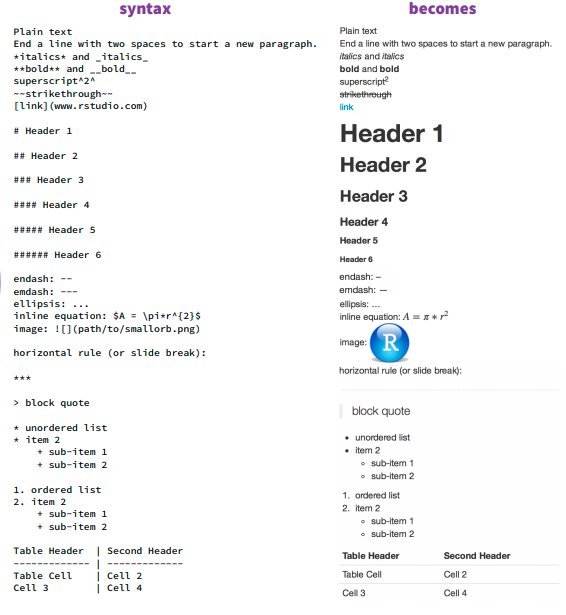
\includegraphics{images/RMD_formatting.png} Bold: `\textbf{' on either
end of a word, phrase, or line will make it bold!} this is in bold**
='\textbf{`this is in bold'}' without the quotes around the **\\

Line breaks: DO you want text to be on different lines? Insert a '\,' at
the end of a line to make a line break!

\hypertarget{making-a-code-chunk}{%
\subsection{\texorpdfstring{\textbf{Making a code
chunk}}{Making a code chunk}}\label{making-a-code-chunk}}

Since qmd documents are text based, we need to tell RStudio when we want
to actually include code. To do this, we will insert a code chunk. To
insert a code chunk:\\

1.) Use the keyboard shortcut `ctrl'+`alt'+`i' (PC) or `cmd'+`alt'+`i'
(Mac) to insert a code chunk.\\

2.) Navigate to the top bar (of the top left quadrant of RStudio), find
``+c'' at the right of the bar to insert an R code chink.

Once you have a code chunk inserted you will notice that the background
of the chunk is gray instead of your default background color (white or
black if you are in dark mode)

\begin{Shaded}
\begin{Highlighting}[]
\CommentTok{\#this is an example code chunk}

\CommentTok{\# Using \textquotesingle{}\#\textquotesingle{} at the start of a line indicates a comment, which is not runnable code!}
\end{Highlighting}
\end{Shaded}

\hypertarget{rendering-your-report}{%
\subsection{\texorpdfstring{\textbf{Rendering your
report}}{Rendering your report}}\label{rendering-your-report}}

To Visualize what your report will look like, click the `visual' tab in
the top bar (on the left). Note that if you do this, it CAN change your
code--so be careful. You can also use the GUI to alter your report in
the visual tab. This provides a nice alternative to the code based
formatting options in the `source' tab.\\

To actually render into an html or pdf document, you must click
``Render''. You can use the arrow to the right of ``Render'' to choose
render to html or render to pdf. I suggest using HTML most of the time
but you can use pdf if you prefer. You will need to successfull Render
your quarto document into an html or pdf report in order to turn in your
labs! :::

\begin{center}\rule{0.5\linewidth}{0.5pt}\end{center}



\end{document}
